\documentclass{sintefbeamer}

% packages, font, color, and newcommands
\usepackage{amsfonts, amsmath, oldgerm, lmodern, bm}
% \usepackage[font={footnotesize}]{caption}
\usepackage{natbib}
\usepackage{url}
\usepackage{tikz}
\usepackage{amssymb}
\usepackage{amsmath}
\usepackage{amsthm}
\usepackage{mathrsfs}
\usepackage{empheq}
\usepackage{mdframed}
\usepackage{bm}
\usepackage{animate}
\usepackage{xcolor,colortbl}
\usepackage{graphicx}
%\usepackage{dot2texi}
% \usepackage{dot2texi}
\usepackage{tikz}
\usetikzlibrary{shapes,arrows}

\bibliographystyle{apalike}
\usefonttheme{serif}
\usetikzlibrary{calc}
\definecolor{carminered}{rgb}{1.0, 0.0, 0.22}
\definecolor{burgundy}{rgb}{0.5, 0.0, 0.13}
\title{Averaged equations for a buoyancy driven suspension of \underline{contaminated} droplets}
\subtitle{Discussion FoReCaSt}
\author{\underline{N. Fintzi} \footnote{IFP \'Energies Nouvelles, France}, and JL. Pierson$^1$}
% \date{Created on May 22, 2022}
\definecolor{burntorange}{rgb}{0.8, 0.33, 0.0}
\titlebackground{image/Hidman.png}


% document body
\addtobeamertemplate{navigation symbols}{}{%
    \usebeamerfont{footline}%
    \usebeamercolor[fg]{footline}%
    % \hspace{1em}%
    % \vspace{1em}%
    \insertframenumber/\inserttotalframenumber
}
\usepackage{stmaryrd}


\begin{document}
\maketitle
\section*{}

\begin{frame}
  \frametitle{Objectives and motivation}



\textbf{Euler-Euler} modeling of dispersed two phase flows 
\vfill
\begin{enumerate}
  \item Study the effect of \textbf{non-uniform surface tension} on the hydrodynamic of the droplet.
  \item The surface tension $\gamma$ is a thermodynamic function of 
  \begin{itemize}
    \item surfactant concentration $\Gamma$  
    \item temperature $T$
  \end{itemize}
  \item Impact of these effect on the continuous phase averaged equation. 
\end{enumerate}
\end{frame}


\begin{frame}
  \frametitle{Isolated droplet in Stokes flow with Marangoni stress}

  \begin{columns}
    \begin{column}{0.33\textwidth}
      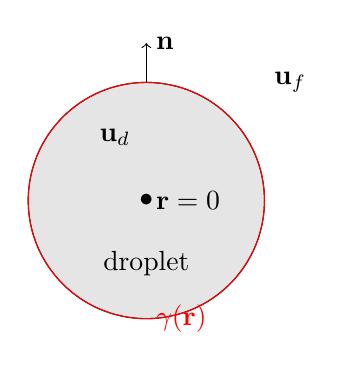
\begin{tikzpicture}
        \draw[fill=gray!20] (0,0) circle (1.5);
        \draw (0,0)node{$\bullet$}node[right]{$\textbf{r}=0$};
        \draw (-0.4,0.8)node{$\textbf{u}_d$};
        \draw (0,-0.8)node{droplet};
        \draw[red] (0,0) circle (1.5);
        \draw[red] (0,-1.5) node[right]{$\gamma(\textbf{r})$};
        \draw (1.5,1.5) node[right]{$\textbf{u}_f$};
        \draw [->] (0,1.5) --++ (0,0.5)node[right]{$\textbf{n}$};
      \end{tikzpicture}    \end{column}
    \begin{column}{0.66\textwidth}
      \underline{The Stokes equations}: 
      \begin{align*}
        \div \textbf{u}_f = 0 &&
        \div \textbf{u}_d = 0 \\
        - \grad p_f + \grad^2 \textbf{u}_f = 0 &&
        - \grad p_d + \grad^2 \textbf{u}_d = 0 
      \end{align*}
      \uncover<2->{
        \underline{Kinematic condition at the interface ($r = 1$)}:
        \begin{align}
          \textbf{u}_f = \textbf{u}_d && \textbf{u}_f\cdot \textbf{n} = 0
        \end{align}
        }
        \uncover<3>{
          \underline{Dynamic condition at the interface ($r = 1$)}:
          \begin{align}
            \textbf{n}\cdot (\bm\sigma_f - \lambda \bm\sigma_d)
            \cdot (\bm\delta - \textbf{nn})
            =\frac{1}{Ca}
            (\bm\delta - \textbf{nn})\cdot \textcolor{red}{\grad \gamma}
          \end{align}
          }

    \end{column}
  \end{columns}
  \begin{itemize}
    % \item<2-> $\textbf{e}$ Dimensionless velocity direction
    \item<3> $\lambda = \mu_d /\mu_f$ is the viscosity ratio. 
    \item<3> $Ca$ is the capillary number assumed small. 
  \end{itemize}
\end{frame}

\begin{frame}
  \frametitle{Approximation of the surface tension gradient}

  

  \begin{columns}
    \begin{column}{0.33\textwidth}
      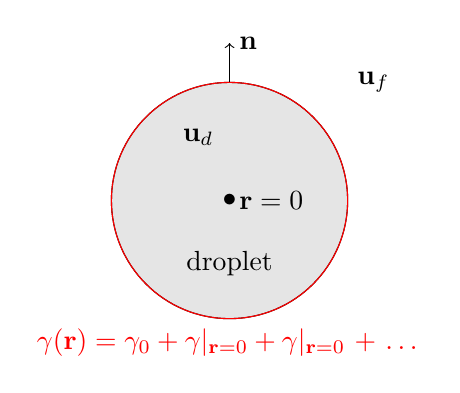
\begin{tikzpicture}
        \draw[fill=gray!20] (0,0) circle (1.5);
        \draw (0,0)node{$\bullet$}node[right]{$\textbf{r}=0$};
        \draw (-0.4,0.8)node{$\textbf{u}_d$};
        \draw (0,-0.8)node{droplet};
        \draw[red] (0,0) circle (1.5);
        \draw[red] (0,-1.5) node[below]{$\gamma(\textbf{r}) = \gamma_0 + \grad \gamma|_{\textbf{r}=0}+ \grad\grad \gamma|_{\textbf{r}=0}$ + \ldots} ;
        \draw (1.5,1.5) node[right]{$\textbf{u}_f$};
        \draw [->] (0,1.5) --++ (0,0.5)node[right]{$\textbf{n}$};
      \end{tikzpicture}    \end{column}
    \begin{column}{0.66\textwidth}
      
          \underline{Dynamic condition at the interface ($r = 1$)}:
          \begin{multline*}
            \textbf{n}\cdot (\bm\sigma_f - \lambda \bm\sigma_d)
            \cdot (\bm\delta - \textbf{nn})\\
            =\frac{1}{Ca}
            (\bm\delta - \textbf{nn})\cdot [\textcolor{red}{\grad \gamma|_{\textbf{r}=0}+ \grad\grad \gamma|_{\textbf{r}=0}}+\ldots]
          \end{multline*}
          

    \end{column}
  \end{columns}

  \vfill
\uncover<2>{
\textbf{The solutions:}  
\begin{itemize}
  \item $\bm\sigma_{f,d} \propto \textcolor{red}{\grad \gamma|_{\textbf{r}=0} \text{ and } \grad\grad \gamma|_{\textbf{r}=0}} \propto \textbf{u}_{f,d}$
  \item $\textbf{u}_{f,d} = \textbf{C}_1(\lambda, \textbf{r})\cdot  \textcolor{red}{\grad \gamma}+ \textbf{C}_2(\lambda, \textbf{r}) : \textcolor{red}{\grad\grad \gamma} + \textbf{C}_3(\lambda, \textbf{r}) \cdot \textbf{e}$ in the limit $Ca\to 0$. 
\end{itemize}
}
\end{frame}


\begin{frame}
  \frametitle{Solution}
\begin{equation}
  \pSavg{ \bm\sigma_f \cdot \textbf{n}}
  =
  \phi \frac{ 1}{2 \left(\lambda + 1\right)}
  \grad \gamma
  % (\times a ?)
\end{equation}
\begin{equation}
  \pSavg{ \textbf{r}\bm\sigma_f \cdot \textbf{n}}
  =
  \phi \frac{ \left(25 \lambda + 14\right)}{25 \left(\lambda + 1\right)}
  \grad\grad \gamma
  % (\times a ?)
\end{equation}
\end{frame}

\begin{frame}
  \frametitle{Conclusion: Averaged continuous phase equations}
\begin{align*}
  &\pddt (\phi_f \rho_f)  
  + \div (
      \phi_f \rho_f\textbf{u}_f
  )
  = 
  0,\\
  &\pddt (\phi_f \rho_f\textbf{u}_f)
  + \div 
      (\phi_f \rho_f\textbf{u}_f\textbf{u}_f)
  = 
  \underbrace{\div \bm\sigma^\text{eff}}_\text{Effective stress}
  + \phi_f \rho_f \textbf{g} 
  \only<1>{- \underbrace{\pSavg{{\bm{\sigma}_f^0 \cdot \textbf{n}_d}}}_\text{Interphase drag force},}
  \only<2>{- \phi \frac{ 1}{2 \left(\lambda + 1\right)} \grad \gamma}
\end{align*}
\pause
\underline{Effective stress: } 
\begin{equation*}
  \bm{\sigma}_f^\text{eff}
  =
  - \underbrace{\avg{\chi_f\rho_f\textbf{u}_f'\textbf{u}_f'}}_\text{Reynolds Stress}
  + \underbrace{\phi_f \bm{\sigma}_f}_\text{Mean Newtonian stress}%- n_p \textbf{M}_p
   \only<1>{+ \underbrace{ {\pSavg{{\textbf{r}\bm{\sigma}_f^0 \cdot \textbf{n}_d}}}}_\text{Stresslet}}
   \only<2>{+ \phi \frac{ \left(25 \lambda + 14\right)}{25 \left(\lambda + 1\right)}
   \grad\grad \gamma}
\end{equation*}


\end{frame}

\end{document}
